%% COMPILATION NOTE 
% uses bibunits package for separate bibliography for appendix
% to compile run 
% pdflatex MRPCalibration  -- creates bu1 bu2 bibliography files
% bibtex bu1
% bibtex bu2
% pdflatex -- again

\documentclass[11pt]{article}

\usepackage[margin=1in]{geometry}
\usepackage{dcolumn}
\usepackage[font=small,labelfont=bf]{caption}
\usepackage{amsmath}
\usepackage{amssymb}
\usepackage{bbm}
\usepackage{rotating}
\usepackage{enumerate}
\usepackage{mathrsfs}
\usepackage{booktabs}
\usepackage{graphicx}
\graphicspath{{../output/figures/}{../output/figures/model-diagnostics/}}
\newcommand{\tabpath}{../output/tables}
\newcommand{\numpath}{../output/tables/numbers-in-text}
\usepackage[hidelinks]{hyperref}
\usepackage{subcaption}
\usepackage[svgnames]{xcolor}
\usepackage{makecell}
\usepackage{adjustbox}

\usepackage[mono=false]{libertine}


% typsetting R code
\usepackage{listings}
\lstset{language=R,
    basicstyle=\small\ttfamily,
    stringstyle=\color{DarkGreen},
    otherkeywords={0,1,2,3,4,5,6,7,8,9},
    morekeywords={TRUE,FALSE},
    deletekeywords={data,frame,length,as,character},
    keywordstyle=\color{black},
    commentstyle=\color{DarkGreen},
}

%% === bibliography packages ===
\usepackage{natbib}
\bibliographystyle{apsr}

% separate appendix bibliography
\usepackage{bibunits}
\defaultbibliographystyle{apsr}     
\defaultbibliography{library,AuxCalibration}



\usepackage{setspace}
\doublespacing
\newcommand{\citepos}[1]{\citeauthor{#1}'s (\citeyear{#1})} % possessive citation


\DeclareMathOperator*{\argmin}{arg\,min} 
\DeclareMathOperator{\E}{\mathbb{E}}
\DeclareMathOperator{\R}{\mathbb{R}}
\DeclareMathOperator*{\N}{\mathcal{N}}
\DeclareMathOperator*{\V}{Var}
\DeclareMathOperator*{\C}{Cov}
\DeclareMathOperator*{\p}{\text{Pr}}
\DeclareMathOperator*{\1}{\mathbbm{1}}
\DeclareMathOperator*{\indp}{\perp\!\!\!\perp}
\DeclareMathOperator{\Lik}{\mathcal{L}}
\DeclareMathOperator{\lik}{\ell}
\DeclareMathOperator{\fishi}{\mathscr{I}}
\DeclareMathOperator{\indsim}{\overset{ind.}{\sim}}
\DeclareMathOperator{\iidsim}{\overset{iid}{\sim}}
\newcommand{\invlogit}{\text{logit}^{-1}}
\newcommand{\mc}[1]{\mathcal{#1}}
\newcommand{\mbf}[1]{\mathbf{#1}}
\newcommand{\bb}[1]{\mathbbm{#1}}


\newtheorem{theorem}{Theorem}
\newtheorem{prop}{Proposition}
\newtheorem{assm}{Assumption}
\newtheorem{remark}{Remark}


% caption goes in \caption{}, notes go underneath table/figure in \capnotes{}
\newcommand{\capnotes}[1]{\footnotesize\caption*{\textit{Notes}: #1}} 
\newcommand{\tinysec}[1]{\medskip\textbf{#1}}
\newcommand{\inputy}[1]{\input{#1}\unskip} % gets rid of space after inputting file

% add extra spacing in enumerate environment
\addtolength{\jot}{.75em}

%% For appendix TOC
\usepackage[toc,page,header]{appendix}
\usepackage{minitoc}
\renewcommand \thepart{} % Make the "Part I" text invisible
\renewcommand \partname{}

% month-year date format
\usepackage{datetime}
\newdateformat{monthyeardate}{%
\monthname[\THEMONTH] \THEYEAR}

% change section header size. conflicts with apx TOC from minitoc
% \usepackage{sectsty}
% \sectionfont{\fontsize{13}{15}\selectfont}
% \subsectionfont{\fontsize{12}{15}\selectfont}
\usepackage{titlesec}
\titleformat{\section}{\normalfont\fontsize{13}{15}\bfseries}{\thesection}{1em}{}
\titleformat{\subsection}{\normalfont\fontsize{13}{15}\bfseries}{\thesubsection}{1em}{}


% Editing modes - mark \todo, \tocheck
\newcommand{\todo}[1]{{\color{red}[#1]}}
\newcommand{\tocheck}[1]{{\color{red}#1 (CHECK THIS)}}


% for blind submission switch this to 1
\newcommand{\blind}{0}


% uncomment to get rid of tables and figures for accurate work count
% \usepackage{environ}
% \RenewEnviron{figure}{}
% \RenewEnviron{table}{}



\title{Improving Small-Area Estimates of Public Opinion by Calibrating to Known Population Quantities
\if0\blind
\thanks{%
	For helpful comments we thank Larry Bartels, Devin Caughey, Shira Mitchell, Jacob Montgomery, John Sides, Matt Tyler, and panelists at the 2023 APSA panel on Developments in Survey Methods. An \texttt{R} package implementing methods proposed in this paper is available for download at \url{http://github.com/wpmarble/calibratedMRP}. 
	}
\fi
}

\if0\blind
	\author{
		William Marble\footnote{Hoover Fellow, Hoover Institution, Stanford University. Email: \href{mailto:wpmarble@stanford.edu}{wpmarble@stanford.edu}}
	 \and 
	 	Josh Clinton\footnote{Abby and Jon Winkelried Chair, Professor of Political Science, Department of Political Science, Vanderbilt University. Email: \href{mailto:josh.clinton@vanderbilt.edu}{josh.clinton@vanderbilt.edu}}}
\fi





\date{\monthyeardate\today}



\begin{document}


%%% Title Page %%%%
\begin{singlespacing}
\maketitle	
\thispagestyle{empty}
\begin{abstract}
Multilevel regression and poststratification (MRP) is widely used to estimate opinion in small subgroups and to adjust unrepresentative surveys.
Yet, even flexible MRP models contain errors generated by non-response and model misspecification.
We propose a principled, data-driven method to leverage observable errors on auxiliary quantities with known marginal distributions --- e.g., election outcomes --- to improve estimates of policy attitudes. 
Our method leverages the correlation between auxiliary variables and outcomes of interest to calibrate MRP estimates to these known marginal distributions.
We illustrate our approach using a pre-election poll measuring support for an abortion referendum. 
We find that the method reduces county-level error by nearly two-thirds relative to traditional MRP.
We also show how our calibration approach can be used to generate estimates for smaller nested geographies, such as precincts, even in the absence of poststratification data at this level.
Our approach provides a framework for fully incorporating known population data to improve estimates of public opinion in small subgroups, providing scholars another tool to study representation.
% ~\\\bigskip
% Word Count: 10,000
\end{abstract}


\end{singlespacing}
\newpage
\clearpage


%%% uncomment for table of contents %%%
% \thispagestyle{empty}\tableofcontents\clearpage

%%% these commands put an "introduction" section in the PDF's metadata
\phantomsection
\addcontentsline{toc}{section}{Introduction}

%%% START OF MAIN TEXT %%%
\setcounter{page}{1}

%% start(appendix TOC)
\doparttoc % Tell to minitoc to generate a toc for the parts
\faketableofcontents % Run a fake tableofcontents command for the partocs
%% end(appendix TOC)

\begin{bibunit}



Surveys are fundamental to the measurement of public opinion and behavior, but the deteriorating performance of both pre-election polls \citep{Cetal:2021,Keta:2016} and academic surveys \citep{Jacobson2022} has fueled concerns that survey respondents differ from the populations they are meant to reflect \citep{PNAS2023,Bailey2023}.
Researchers have proposed several methods to address these concerns. 
A particularly important approach is multilevel regression and poststratification (MRP) \citep{GL:1997,PGB:2004}, which combines regression modeling with poststratification to estimate opinion in populations that were not intentionally sampled.

Despite these improvements, MRP estimates may still suffer from at least three sources of error: (1) nonignorable nonresponse, where respondents differ from nonrespondents in ways not captured by covariates \citep[e.g.,][]{CLT:2022}; (2) poststratification error, where population targets are proxied or measured with error; and (3) model specification error and sampling variation.

These errors matter: a rich literature uses constituency-level opinion estimates to assess democratic representation, but interpreting discrepancies between public opinion and policy as ``democratic deficits'' \citep{LP:2012} requires confidence that these gaps are not artifacts of survey error --- confidence that is increasingly difficult to justify \citep{C:2022}.\footnote{Work on this question extends back at least to \citet{MS:1963} and \citet{A:1978}.  More recently, see: \citet{Gelman2009,LP:2012,LPJ:2008,C:2006,TW:2013,T:2015,CW:2022,SP:2023,BS:2018,HFMS:2019}.
Other closely related work involves studying subgroup opinion and behavior within electoral districts \citep{GG:2013,Kuriwaki2023,LS:2019,WR:2012}.}

A large literature has proposed MRP-related strategies to improve small-area opinion measurement \citep{GG:2013,HanrettyLauderdaleVivyan2016,LW:2017,B:2019,CW:2019,Ornstein2020,BruchFelderer2022, BLW:2022,G:2023,BMFH:2023, RMO:2023}.
We contribute a method that reduces both the bias and variance of MRP estimates by leveraging auxiliary data with known marginals (e.g., election results) to calibrate estimates of correlated outcomes lacking ground truth (e.g., policy attitudes).

The core insight is that because attitudes are correlated across issues, so too are errors in survey-based estimates: if an MRP model overestimates Democratic vote share in a county, it probably also overestimates support for increasing the minimum wage.
Our approach jointly models outcomes of interest alongside auxiliary variables with known ground truth, estimating the geographic-level correlations across variables.
We then use these estimated correlations to update estimates of target variables based on the observed calibration error for the auxiliary variables with ground-truth data.
This approach, which is agnostic as to the source of error, provides larger adjustments for more highly correlated variables.
Our method also enables opinion estimation in smaller geographies than those in the survey or poststratification data by applying calibration at a lower, nested level (e.g., precincts within counties).
We implement our methods in \texttt{R} software available at \url{http://github.com/wpmarble/calibratedMRP}.\footnote{Appendix \ref{apx:software} demonstrates key functionality.}

We validate our approach using pre-election polling in the 2022 Michigan midterm election.
We focus on elections for governor, secretary of state, and a ballot proposition on reproductive rights (Proposition 3).
Calibrating to the governor race reduces county-level error by about two-thirds in the other elections.
Our precinct-level extension reduces error by 60\%.
Simulations show that the procedure is most helpful when the calibration variable is highly correlated with the outcome of interest, and that it substantially reduces error even with small, highly non-representative samples.

Methodologically, we build on methods for calibrating model-based inferences to known population quantities.
MRP researchers commonly use a ``logit shift'' to adjust discrepancies between known aggregates and model-based estimates \citep{GG:2013,RMO:2023}.\footnote{For example, \citet{Kuriwaki2023} are interested in the distribution of vote choice by racial group within each congressional district. While ground truth data on racial voting is not available, they apply the logit shift to district aggregates to ensure their estimates are consistent with known election results.}
We extend this approach by jointly modeling correlated outcomes and exploiting their covariance structure to improve estimates for outcomes with unobserved true values.
Our work is also related to efforts to expand poststratification using synthetic targets \citep{LW:2017}; our approach sidesteps synthetic poststratification tables entirely, requiring only marginal distributions of auxiliary variables at the geographic level of interest.




\section{Survey Adjustment Using Multilevel Regression and Poststratification}
\label{sec:mrp-overview}
MRP involves three steps. First, researchers use survey data to estimate a regression model predicting an outcome of interest (e.g., opinion, behavior). 
The regression includes individual- and geographic-level predictors whose joint distribution is known (e.g., from Census microdata). 
Second, the model predicts the expected outcome for each combination of covariates in the known joint distribution (i.e., each poststratification cell). Third, final estimates are weighted averages of predicted outcomes in each cell.
The weights are proportional to population size of the cell.\footnote{We will often refer to the subgroup of interest as a ``geography,'' following  work employing MRP to estimate opinion in sub-national political units. It is important to note, however, that MRP can be applied just as easily to other subgroups, such as those defined by race or age, so long as their joint distribution with other variables in the regression is known. }

\subsection{Population Quantities}

Suppose we are interested in public opinion on $J$ binary outcomes. Our estimands $\theta^j$ denote the population share holding attitude $j$. Superscripts index issues; subscripts index groups or individuals.
For example, $\theta^j$ might represent the share of the public who turn out to vote, who vote for the Democrat, or who support a policy.

The population is partitioned into a set of cells $\mathcal{C}$, where each cell $c$ is defined by a combination of demographic variables and geography. 
For example, $\mathcal{C}$ might represent every combination of age, race, gender, education, and county. 
Population cell sizes $N_c$ are known from Census data or other sources.\footnote{When researchers do not have information on the full joint distribution, there are several methods available to estimate the joint distribution. Key ideas in the literature include combining marginal distributions by assuming independence, using survey data to estimate the joint distribution, or combining these two approaches \citep{LW:2017,CW:2019}.\label{fn:synthps}}  
The total population is the sum of cell populations: $N \equiv \sum_c N_c$. 
The poststratification table is defined by cell-level covariates and cell sizes $N_c$.
Because cells are defined by geography, let $\mathcal{C}_g$ denote the cells within geography $g$ (e.g., $\mathcal{C}_{\text{Calif.}}$ for California).

Population opinion is a weighted average of cell-level opinion:
\begin{align}
\begin{split}
	\text{population-level opinion:} \quad &\theta^j \equiv \frac{\sum  N_c \theta_c^j}{\sum N_c} \\
	\text{opinion in geography $g$:} \quad &\theta_g^j \equiv \frac{\sum_{c \in \mathcal{C}_g}  N_c \theta_c^j}{\sum_{c \in \mathcal{C}_g} N_c} 
	\label{eq:popopinion}
\end{split}
\end{align}

\subsection{MRP Estimation}

MRP estimation proceeds by using survey data to fit a regression model for $\theta^j_c$ as a function of covariates in the poststratification table.
The model typically includes geographic intercepts to capture remaining between-geography variation after accounting for individual-level covariates.
The model is used to generate predictions $\hat{\theta}^j_c$ for each cell.
After generating opinion estimates for each cell, researchers then poststratify those estimates to the geography of interest ---  i.e., substituting estimates for the population quantities in Equation~\ref{eq:popopinion}.

MRP allows researchers to estimate opinion in geographies that were not intentionally sampled. 
For example, researchers studying representation may want to know whether policy outcomes accord with public opinion \citep[e.g.,][]{LP:2012,Tausanovitch2014}, but even large surveys are unlikely to have many respondents in any given geography.
MRP provides a solution by pooling information across geography and demographics via the regression step and accounting for differences in population composition via the poststratification step. 

\subsection{Remaining Sources of Error}

The performance of the MRP estimates relies on ignorability: conditional on covariates, representation in the survey is independent of the outcome.
Under ignorability and correct model specification, MRP is consistent.
To make these assumptions more plausible, recent work has focused on specifying more complex interactions \citep[e.g.,][]{GG:2013,B:2019,BLW:2022,G:2023} and increasing the number of poststratification variables \citep{LW:2017}.
Still, respondents may differ from non-respondents in unobservable ways. Additionally, attempts to reduce bias by increasing model complexity may be offset by increased variance \citep{BH:2013,WR:2012}.

A second source of error arises when the population of interest differs from the population used to construct the poststratification table.
An example is estimating the opinions of the electorate using the voting-age population demographics.  

Finally, even under ideal conditions, MRP does not guarantee accurate estimates for every geography: model-based estimates that are unbiased overall can still produce sizable errors in specific areas.





\section{Calibrating a Single Outcome to Ground-Truth Data}
\label{sec:singleadjust}

The quality of MRP inference depends on how well the regression is able to model opinion within each cell.
Researchers can sometimes assess error by comparing model-based estimates to known quantities --- typically in the context of election surveys.
We do not know how particular individuals voted, but we do know election outcomes at various levels of geographic aggregation. 
Even if predicting opinion in these geographies is not of primary interest, these discrepancies can be used to  improve inference for other subgroups. 

A popular method of adjusting MRP estimates to account for such error involves adding a geography-specific intercept shift to the modeled probabilities in each poststratification cell.\footnote{In Appendix~\ref{apx:otherwting}, we review how to account for this information in a classic survey weighting context and discuss limitations to that approach.}  
The values of these geographic intercepts are chosen such that the model-implied vote shares exactly match the known population vote shares in each geographic unit \citep[769]{GG:2013}.
Because the intercept adjustment is applied on the logit scale, this method has been called the ``logit shift.''

To formalize this method, suppose we observe the population-level outcome $\theta_g^j$ for some geography $g$. 
Given model estimates $\hat{\theta}_g^j$, we calibrate results by adding an intercept shift on the logit scale to the predicted probabilities.
The logit shift parameter for geography $g$ on outcome $j$ is the value of $\delta_g^j$ that solves:
\begin{align}
	\underbrace{\theta_g^j}_{\substack{\text{ground truth} \\ \text{for geography $g$}}} &= \,\, \underbrace{\frac{1}{N_g} \sum_{c \in \mathcal{C}_g} N_c \,\, \overbrace{\text{logit}^{-1}\left(\delta_{g[c]}^j + \text{logit}(\hat{\theta}_c^j) \right)}^{\text{updated estimate for cell $c$}}}_{\text{updated estimate for geography $g$}}, \label{eq:logitshift}
\end{align}
where $N_g \equiv \sum_{c \in \mathcal{C}_g} N_c$ is the population of geography $g$ and the notation $g[c]$ indicates the geography for cell $c$.
This expression equates the adjusted model-implied outcome to the ground-truth population outcome $\theta_g^j$. 

The new cell-level probabilities are generated by applying the geographic offset to the existing probabilities: 
\begin{align}
	\tilde{\theta}_c^j = \text{logit}^{-1}\left( \delta_{g[c]}^j + \text{logit}(\hat{\theta}_c^j)\right). \label{eq:updatedprobs}
\end{align}
When the updated estimates are poststratified to the geographic level, they exactly match the ground-truth data. 
When poststratified to other subgroups, the results will generally differ from the uncalibrated MRP results.

For example, researchers studying racially polarized voting may estimate an MRP model, apply the logit shift at the district level to match actual election results, and aggregate adjusted estimates to the racial-group level \citep{Kuriwaki2023}. The resulting race-level vote share estimates will differ from their uncalibrated counterparts.

The logit shift is a minimal, geographic-based adjustment that does not distinguish between individuals within the same geography and has been shown to approximate the posterior distribution of cell-level probabilities conditional on the ground truth \citep{RMO:2023}.



Calibration improves estimates only under certain assumptions \citep[section 3]{RMO:2023}. The shift is uniform within each geography, so if the true error is not uniform, calibration may increase error for some cells even as it decreases average error.
The uniform-shift assumption is more appropriate for homogeneous geographies. Given residential segregation along political and racial lines \citep{Rodden2019}, the logit shift generally works better at smaller scales.


\section{Adjusting Multiple Outcomes to Account for Ground-Truth Data}
\label{sec:multiadjust}
\input{sections/multiadjust}

\section{Validation in Michigan Elections in 2022}
\label{sec:validation}
The primary use case for this method is measuring public opinion on policy issues. Evaluating the method requires: (1) a policy issue with available ground-truth data; and (2) a survey measuring that issue alongside variables suitable for calibration. 

We evaluate the method using pre-election polling of the 2022 Michigan midterm election.
This election featured a referendum concerning abortion rights (Proposition 3) alongside races for Governor and Secretary of State. 
We calibrate to ground-truth Governor and Secretary of State results and evaluate how this changes estimates of Proposition 3 opinion.



We use data from an original survey conducted via SurveyMonkey in fall 2022.\footnote{Because no sensitive information was collected, the IRB \if0\blind at the University of Pennsylvania~\fi deemed the survey exempt from review\if0\blind~(Protocol \#852133)\fi.} 
Respondents were recruited via a river sample: users who completed any SurveyMonkey survey during this period were invited to take a survey on the 2022 midterm elections.
We have $N =\inputy{\numpath/michigan-sample-size.txt}$ Michigan respondents who answered all demographic and outcome questions.
Appendix \ref{apx:modeling} contains details of this case and survey. 


\subsection{Validation Approach}

We model vote choice for the three statewide elections (alongside other opinions) as a function of respondent- and county-level predictors.
We first generate uncalibrated county-level estimates by poststratifying on the joint distribution of county demographics.  
We then calibrate to observed county-level margins for the Governor and Secretary of State races and assess how this changes estimation error.

Individual-level predictors include age, race, gender, education, with interactions between race $\times$ education and nonwhite $\times$ education $\times$ age.
County-level predictors are percent nonwhite, percent Hispanic/Latino, percent college-educated, median income, and 2020 Biden two-party vote share. 
The specification includes county-level random intercepts correlated across outcomes, which provide the basis for our adjustment.
Further modeling details, including \texttt{R} code, are included in Appendix \ref{apx:modeling}.\footnote{Additionally, Appendix \ref{apx:priors} examines the sensitivity of our results to the choice of prior distributions.}

We produce two sets of adjusted results: the first calibrates Secretary of State and Proposition 3 using gubernatorial results; the second calibrates Proposition 3 using both gubernatorial and Secretary of State results.

Because we calibrate to two-party vote share, the calibration implicitly targets the \textit{electorate} rather than the \textit{population}. 
The approach can target the population instead by including turnout as a calibration variable --- i.e., calibrating to Democratic vote share, Republican vote share, and aggregate turnout as functions of total population. 
We take this approach in a simulation study in Appendix \ref{apx:simulations}.
Researchers should take care in specifying the population of interest --- which depends on the substantive research question --- and ensuring that the calibration variables are measured accordingly.



\subsection{Validation Results}

Calibration substantially reduces error: average absolute error for Secretary of State and Proposition 3 falls by \inputy{\numpath/sos-mae-reduction.tex} and \inputy{\numpath/prop3-mae-reduction.tex}, respectively. % calculated from tab:mi-cty-error


Table~\ref{tab:mi-cors} reports correlations between county-level random intercepts across outcomes. This matrix measures residual within-county correlation on the logit scale after accounting for covariates.

\begin{table}[tb]
	\centering
	\caption{Correlation of County Intercepts Across Outcomes, Michigan 2022}
	\label{tab:mi-cors}
	\resizebox{\textwidth}{!}{
\begin{tabular}{l>{\raggedleft\arraybackslash}p{2cm}>{\raggedleft\arraybackslash}p{2cm}>{\raggedleft\arraybackslash}p{2cm}>{\raggedleft\arraybackslash}p{2cm}>{\raggedleft\arraybackslash}p{2cm}>{\raggedleft\arraybackslash}p{2cm}>{\raggedleft\arraybackslash}p{2cm}>{\raggedleft\arraybackslash}p{2cm}>{\raggedleft\arraybackslash}p{2cm}}
\toprule
  & Governor & Secretary of State & Abortion Prop. & Biden Legitimate & Biden Approval & Fair Elections & Democratic PID & Independent PID & Republican PID\\
\midrule
Governor & 1.00 &  &  &  &  &  &  &  & \\
Secretary of State & 0.69 & 1.00 &  &  &  &  &  &  & \\
Abortion Prop. & 0.70 & 0.68 & 1.00 &  &  &  &  &  & \\
Biden Legitimate & 0.69 & 0.66 & 0.68 & 1.00 &  &  &  &  & \\
Biden Approval & 0.68 & 0.65 & 0.68 & 0.68 & 1.00 &  &  &  & \\
Fair Elections & 0.62 & 0.59 & 0.60 & 0.67 & 0.62 & 1.00 &  &  & \\
Democratic PID & 0.62 & 0.57 & 0.60 & 0.61 & 0.60 & 0.56 & 1.00 &  & \\
Independent PID & -0.06 & -0.01 & -0.03 & -0.08 & -0.05 & -0.11 & -0.24 & 1.00 & \\
Republican PID & -0.49 & -0.50 & -0.49 & -0.46 & -0.47 & -0.40 & -0.37 & -0.22 & 1\\
\bottomrule
\end{tabular}}
	\capnotes{Posterior mean correlations between county random intercepts across survey outcomes.}
\end{table}

Consistent with partisan and geographic sorting, county intercept correlations are relatively high across outcomes.
The sole exception is independent party identification, which is largely unrelated to other county-level opinions.

Despite these high average correlations, Table \ref{tab:mi-cors} reveals interesting variation. 
For example, the residual geographic correlation between governor vote choice and belief that Biden won legitimately is just below $0.7$, but the correlation between governor vote choice and Republican party identification is about $-0.5$. 
Calibrating to gubernatorial results will thus produce a smaller update for party identification than for beliefs about Biden's legitimacy.
In short, gubernatorial vote choice carries more information about opinions on Biden's legitimacy than about party identification.
This is consistent with the specifics of the race: Republican gubernatorial candidate Tudor Dixon denied Biden's 2020 victory, alienating some Republicans \citep{U:2022}. 

Using these correlations, we calibrate to outcomes with known county-level values. 
Figure~\ref{fig:mi-cty-elec-rs} plots true county-level vote share against: (1) uncalibrated MRP estimates; (2) estimates calibrated to gubernatorial results; and (3) estimates calibrated to both gubernatorial and Secretary of State results.

\begin{figure}[tb]
	\centering
	\caption{County-Level MRP Results, Michigan 2022 Elections}
	\label{fig:mi-cty-elec-rs}
	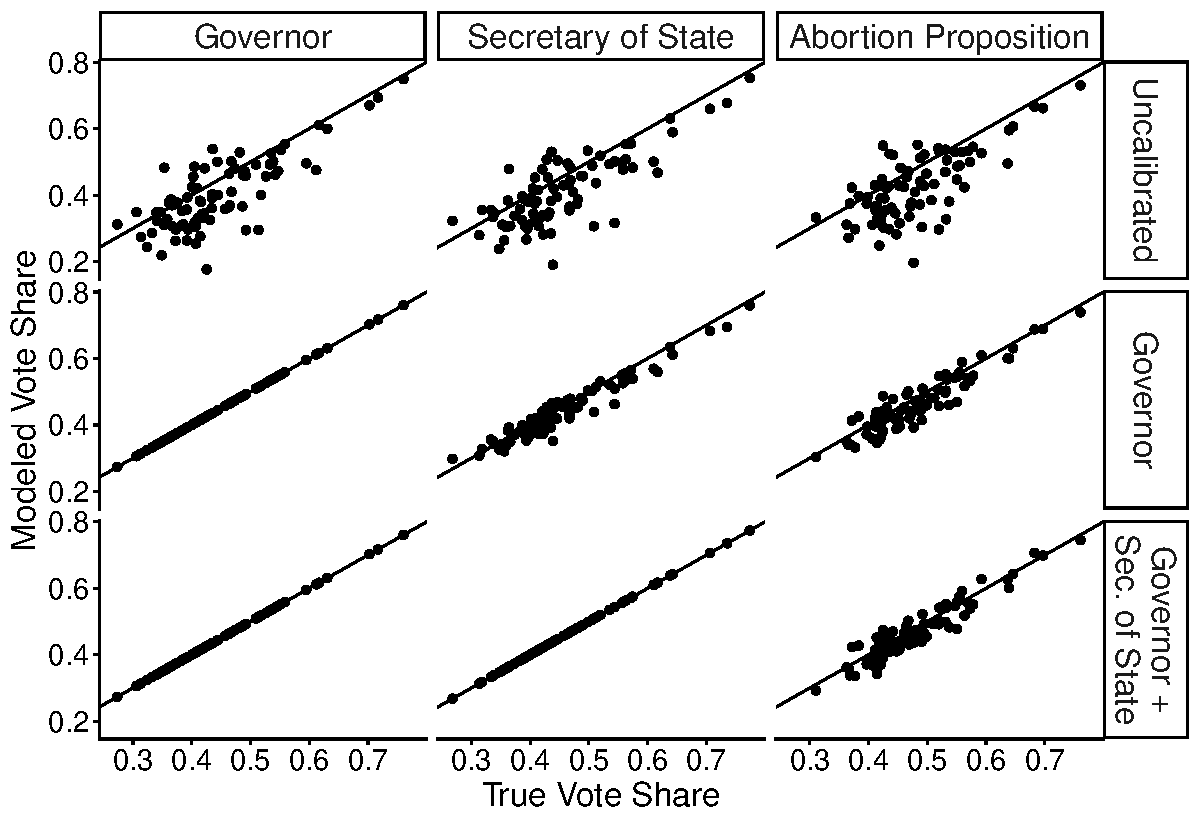
\includegraphics[scale=.7]{mi-elections.pdf}
	\capnotes{The $x$-axis shows the true county-level Democratic/pro-choice vote share and the $y$-axis shows model-based estimates. The top row shows uncalibrated MRP estimates, the middle row shows estimates calibrated to the Governor race, and the bottom row shows estimates calibrated to Governor and Secretary of State races.}
\end{figure}

The top row shows that uncalibrated MRP underestimates Democratic vote share in the gubernatorial and Secretary of State races, as well as the pro-choice position in Proposition 3. 
Moreover, there is evidence of heteroskedasticity, with more variation in polling errors in less-Democratic counties.
Some errors in less-Democratic counties exceed 10 percentage points.

The second row shows the effect of calibrating to gubernatorial results, showing a dramatic improvement in accuracy.
By construction, calibrated gubernatorial vote shares perfectly match actual outcomes (far left). 
The center and right panels show that Secretary of State and Proposition 3 predictions also improve substantially. 
Calibrated estimates are closer to the 45-degree line and heteroskedasticity is greatly reduced. 

The final row shows calibration using both Governor and Secretary of State results.
As the panel in the lower-right reveals, the doubly-calibrated estimate is slightly improved  relative to the estimates calibrated using only the gubernatorial results. 
The mild gains likely reflect the similar relationships both elections have with Proposition 3 support. 
The correlation of county intercepts between the Governor and Secretary of State races was nearly 0.7, indicating that the latter race adds relatively little additional information. 

\begin{table}[tb]
	\centering
	\caption{County-Level Errors,  Michigan 2022 Elections}
	\label{tab:mi-cty-error}
	
\begin{tabular}{rrrrrrr}
\toprule
Race & \makecell[r]{Calibration\\Target} & \makecell[r]{Mean\\Signed Error} & \makecell[r]{Mean\\Abs. Error} & \makecell[r]{Root Mean\\Sq. Error} & \makecell[r]{Min.\\Error} & \makecell[r]{Max.\\Error}\\
\midrule
Governor & None & $-4.4$ & $6.2$ & $8.0$ & $-24.9$ & $12.9$\\
 & Governor & $-$ & $-$ & $-$ & $-$ & $-$\\
 & \makecell[l]{Governor +\\Sec. of State} & $-$ & $-$ & $-$ & $-$ & \vphantom{1} $-$\\
\midrule
\addlinespace
\makecell[r]{Secretary\\of State} & None & $-4.5$ & $6.2$ & $7.9$ & $-24.8$ & $11.4$\\
 & Governor & $-1.4$ & $2.2$ & $2.8$ & $ -8.7$ & $ 3.0$\\
 & \makecell[l]{Governor +\\Sec. of State} & $-$ & $-$ & $-$ & $-$ & $-$\\
\midrule
\addlinespace
Abortion Proposition & None & $-5.5$ & $7.0$ & $8.9$ & $-28.0$ & $12.4$\\
 & Governor & $-1.7$ & $2.8$ & $3.5$ & $ -8.4$ & $ 6.2$\\
 & \makecell[l]{Governor +\\Sec. of State} & $-1.0$ & $2.4$ & $2.9$ & $ -7.3$ & $ 5.1$\\
\bottomrule
\end{tabular}
	\capnotes{Entries in the table show the county-level error associated with uncalibrated and calibrated MRP vote share estimates for the Democrat/pro-choice outcome. The first row for each race is the error when using uncalibrated MRP; the second row is the error when calibrating to the governor outcomes; the third row is the error when calibrating to both the Governor and Secretary of State outcomes.}
\end{table}

Table~\ref{tab:mi-cty-error} summarizes these results by calculating the mean signed error, the mean absolute error (MAE), the root mean squared error (RMSE), and the range of errors across counties. 
Each panel has three rows: uncalibrated MRP, calibrated to Governor, and calibrated to both Governor and Secretary of State. 

Calibrating to the Governor race reduces mean signed error in the Secretary of State race from {\inputy{\numpath/sos-msgnederror-uncalib.tex}} percentage points in the Republican direction to just {\inputy{\numpath/sos-msgnederror-calib-gov.tex}}  points --- a reduction of {\inputy{\numpath/sos-msnederror-reduction.tex}}.
MAE and RMSE both fall by nearly two-thirds and the error range shrinks dramatically, from {\inputy{\numpath/sos-error-range-uncalib.tex}} to {\inputy{\numpath/sos-error-range-calib-gov.tex}}.

Proposition 3 results show modest additional gains from calibrating to multiple outcomes. 
The MAE is reduced from {\inputy{\numpath/prop3-mae-uncalib.tex}} to {\inputy{\numpath/prop3-mae-calib-gov.tex}} percentage points when calibrating to the Governor results --- a reduction of {\inputy{\numpath/prop3-mae-reduction.tex}}.  
Jointly calibrating to both races further reduces the MAE to {\inputy{\numpath/prop3-mae-calib-gov-sos.tex}} percentage points. 
Maximum and minimum errors are also greatly reduced by calibrating to both races.

\begin{figure}[tb]
	\centering
	\caption{Change in County-Level Estimates from Calibration to Governor Results}
 	\label{fig:mi-change-error}
 	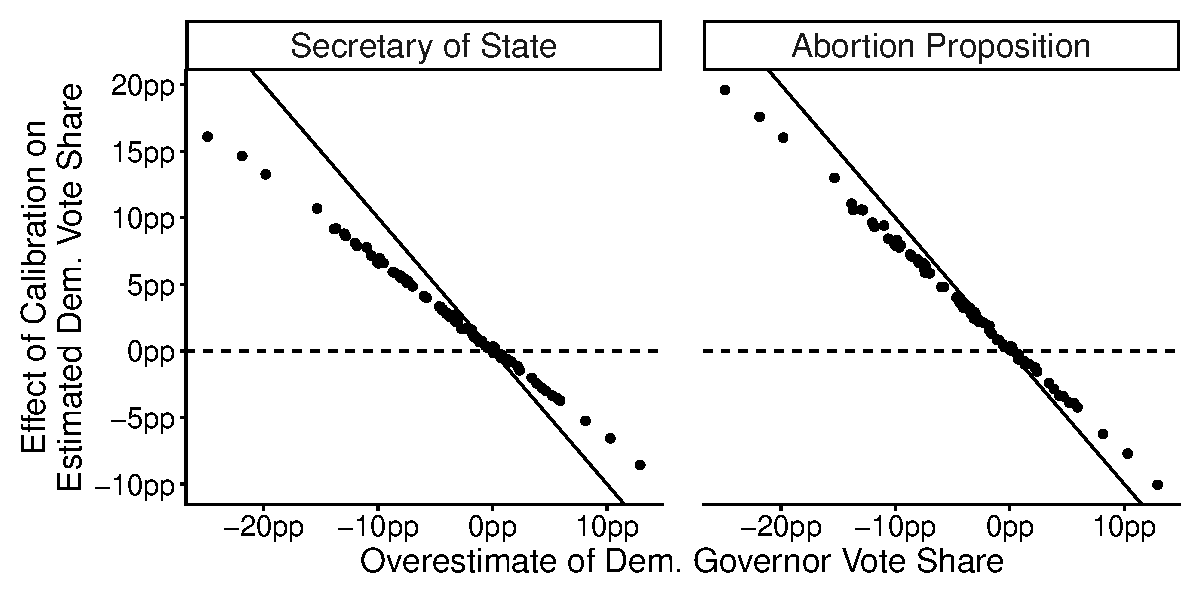
\includegraphics[scale=.75]{mi-calib-adjustment-by-gov-error.pdf}
 	\capnotes{The $y$-axis plots the difference between calibrated and uncalibrated county-level estimates for Secretary of State and the abortion proposition. The $x$-axis shows the county-level error in the Governor's race before calibration where positive values indicate overestimating the support for Democratic incumbent Gretchen Whitmer.}
\end{figure}


To visualize the nature of the calibration, Figure \ref{fig:mi-change-error} plots the effect of calibration in the Secretary of State and abortion proposition against the baseline error in estimates for Governor.\footnote{Figure \ref{fig:mi-change-result} in the Appendix plots the calibration effect against the raw county-level Governor results.}
The $x$-axis shows the gubernatorial overestimate; the $y$-axis shows the change in estimates after calibration.

The pattern is intuitive: where standard MRP overestimates gubernatorial Democratic vote share, other estimates are revised downward.
Most points fall below 0 on the $x$-axis --- indicating that baseline MRP underestimates Democratic vote share.
Consequently, most observations fall above 0 on the $y$-axis.

The slope reflects the cross-race correlations. One-for-one adjustment would place points on the 45-degree line. The observed slope is flatter, reflecting imperfect correlations across races.
The fact that the left-hand panel has a flatter slope than the right-hand panel reflects the lower correlation  between the Governor and Secretary of State races than between the Governor race and the abortion proposition.

In sum, we find that our calibrated MRP approach can significantly improve estimates of small-area opinion.
We compare our approach to alternatives in Appendix \ref{apx:mrsp}, finding that our method outperforms alternatives in this setting. 
In Appendix \ref{apx:pid}, we also show the effect of calibration on party identification --- an outcome with no ground-truth data in Michigan.
 



\section{Conclusion and Implications}
\label{sec:conclusion}
\input{sections/conclusion}


\clearpage
\begin{singlespace}
% \bibliography{library.bib,AuxCalibration.bib}
  \renewcommand{\refname}{References} % article class; for book/report use \bibname
  \putbib  % uses \defaultbibliography and \defaultbibliographystyle

\end{singlespace}
\end{bibunit}


\begin{bibunit}

%%%%% APPENDIX %%%%%$
\clearpage
\appendix
\singlespacing
\setcounter{page}{0}
\thispagestyle{empty}
\addcontentsline{toc}{section}{Appendix} % Add the appendix text to the document TOC
\vspace*{-1em}
{\centering
\LARGE\bfseries Improving Small-Area Estimates of Public Opinion\\ by Calibrating to Known Population Quantities\par
\bigskip
\Large\normalfont William Marble and Josh Clinton\par
\vspace*{-1em}
}
\part{Appendix} % Start the appendix part
\parttoc % Insert the appendix TOC
\renewcommand\thefigure{\thesection\arabic{figure}}    
\renewcommand\thetable{\thesection\arabic{table}}    
\setcounter{figure}{0}
\setcounter{table}{0}
\setcounter{footnote}{0}
\newpage

\input{sections/appendix}
	

  \clearpage
  \renewcommand{\refname}{Appendix References} % heading for the appendix bib
  \putbib
\end{bibunit}

\end{document}




